\section{Experimentación}

% Descripción de los casos del problema empleados y de los valores de los parámetros considerados en las ejecuciones de cada algoritmo (incluyendo las semillas utilizadas).
% o Resultados obtenidos según el formato especificado.

% Greedy: Si recorres en cada iteración los índices en el mismo orden la infeasiblity siempre será igual hasta que haya un elemento con dos clústers con igual inf, en ese caso si el centroide ha cambiado es posible que cambie de clúster.
% Esto hace que los cambios sean mínimos entre cada iteración, y más probable que termine.

% Si al greedy no descartamos la solución de la iteración anterior conseguimos resultados mucho mejores ?
% Se ha creado una segunda versión en la que no se descarta la solución anterior, y se calcula la inf en toda la solución
% Se ha creado una tercera en la que el cálculo de las distancias es -> Mejor olvidarse de esta

\vspace*{\fill}

\begin{center}
    \begin{tabular}{|| c | c ||} 
        \hline
        \multicolumn{2}{|c|}{\textbf{Semillas}} \\
        \hline
        Ejecución 1 & 949004259 \\
        \hline
        Ejecución 2 & 589741062 \\
        \hline
        Ejecución 3 & 277451237 \\
        \hline
        Ejecución 4 & 49258669 \\
        \hline
        Ejecución 5 & 3773969821 \\
        \hline
    \end{tabular}
\end{center}

\begin{table}[H]
    \centering
    \resizebox{0.85\columnwidth}{!}{%
    \makebox[\textwidth][c]{
    \begin{tabular}{|| c || c ||}
        \hline
        & Agregado \\        
        \hline\hline
        BL & 26.63 \\
        \hline
        COPKM v1 & 14.67 \\
        \hline
        COPKM v2 & 12.69 \\
        \hline
        AGG-UN & 12.17 \\
        \hline
        AGG-SF & 13.62 \\
        \hline
        AGE-UN & 27.94 \\
        \hline
        AGE-SF & 29.24 \\
        \hline
        AM-(10,1.0) & 
        12.43
        \\
        \hline
        AM-(10,0.1) & 
        13.77
        \\
        \hline
        AM-(10,0.1mej) & 
        13.09
        \\
        \hline
    \end{tabular}
    }
    }
    \caption{Valores medios del agregado para cada algoritmo}
\end{table}

\vspace*{\fill}
\newpage
\vspace*{\fill}

\begin{table}[H]
    \centering
    \resizebox{0.83\columnwidth}{!}{%
    \makebox[\textwidth][c]{
    \begin{tabular}{|| c || c c c c || c c c c || c c c c || c c c c ||} 
        \hline
        & \multicolumn{4}{|c||}{Iris} & \multicolumn{4}{|c||}{Ecoli} & \multicolumn{4}{|c|}{Rand} & \multicolumn{4}{|c|}{Newthyroid} \\
        \hline
        & TasaC & TasaInf & Agr & T & TasaC & TasaInf & Agr & T & TasaC & TasaInf & Agr & T & TasaC & TasaInf & Agr & T \\
        \hline\hline
        BL & 0.92 & 141.20 & 1.82 & 27.50 & 46.74 & 1212.80 & 79.28 & 733.33 & 1.12 & 106.00 & 1.88 & 29.21 & 14.16 & 296.80 & 25.02 & 132.10 \\
        \hline
        COPKM v1 & 0.67 & 3.60 & 0.56 & 2.24 & 37.04 & 201.40 & 42.44 & 432.70 & 0.77 & 6.20 & 0.81 & 1.60 & 14.30 & 144.20 & 19.57 & 6.18 \\
        \hline
        COPKM v2 & 0.67 & 0.00 & 0.67 & 2.44 & 37.50 & 57.20 & 39.01 & 117.84 & 0.76 & 0.00 & 0.76 & 2.02 & 14.29 & 0.00 & 14.29 & 6.88 \\
        \hline
        COPKM v2 & 0.67 & 0.00 & 0.67 & 2.44 & 37.50 & 57.20 & 39.01 & 117.84 & 0.76 & 0.00 & 0.76 & 2.02 & 14.29 & 0.00 & 14.29 & 6.88 \\
        \hline
        AGG-UN & 
        0.67 & 0.00 & 0.67 & 126.31 & 24.85 & 208.00 & 30.43 & 492.50 & 0.72 & 2.20 & 0.74 & 125.32 & 11.94 & 59.80 & 14.13 & 219.31
        \\
        \hline
        AGG-SF & 
        0.67 & 0.00 & 0.67 & 115.38 & 28.30 & 380.20 & 38.50 & 450.45 & 0.72 & 0.00 & 0.72 & 115.90 & 12.98 & 45.60 & 14.65 & 201.60
        \\
        \hline
        AGE-UN & 
        0.84 & 119.60 & 1.60 & 12.35 & 41.41 & 1374.80 & 78.30 & 35.30 & 0.97 & 63.00 & 1.43 & 12.31 & 15.77 & 373.72 & 32.54 & 18.53
        \\
        \hline
        AGE-SF & 
        0.87 & 148.20 & 1.81 & 13.00 & 42.31 & 1420.40 & 80.42 & 36.48 & 1.25 & 141.00 & 2.27 & 13.21 & 15.05 & 549.20 & 35.13 & 19.20
        \\
        \hline
        AM-(10,1.0) & 
        0.67 & 0.00 & 0.67 & 180.30 & 26.08 & 171.40 & 30.68 & 706.73 & 0.72 & 4.40 & 0.76 & 182.13 & 13.01 & 53.80 & 14.98 & 313.52
        \\
        \hline
        AM-(10,0.1) & 
        0.67 & 0.00 & 0.67 & 139.89 & 28.46 & 269.40 & 35.69 & 640.27 & 0.72 & 0.00 & 0.72 & 138.58 & 13.58 & 104.00 & 17.38 & 257.87
        \\
        \hline
        AM-(10,0.1mej) & 
        0.67 & 0.00 & 0.67 & 137.71 & 26.33 & 252.20 & 33.09 & 648.11 & 0.72 & 0.00 & 0.72 & 138.53 & 13.36 & 73.40 & 16.05 & 252.86
        \\
        \hline
    \end{tabular}
    }
    }
    \caption{Resultados medios de todos los algoritmos para 10\% de restricciones}
\end{table}

\begin{table}[H]
    \centering
    \resizebox{0.83\columnwidth}{!}{%
    \makebox[\textwidth][c]{
    \begin{tabular}{|| c || c c c c || c c c c || c c c c || c c c c ||} 
        \hline
        & \multicolumn{4}{|c||}{Iris} & \multicolumn{4}{|c||}{Ecoli} & \multicolumn{4}{|c|}{Rand} & \multicolumn{4}{|c|}{Newthyroid} \\
        \hline
        & TasaC & TasaInf & Agr & T & TasaC & TasaInf & Agr & T & TasaC & TasaInf & Agr & T & TasaC & TasaInf & Agr & T \\
        \hline\hline
        BL & 0.90 & 264.80 & 1.74 & 40.18 & 46.85 & 2175.20 & 76.03 & 1242.45 & 1.15 & 293.20 & 2.21 & 38.25 & 14.54 & 576.20 & 25.08 & 182.36 \\
        \hline
        COPKM v1 & 0.67 & 3.40 & 0.68 & 3.55 & 35.08 & 169.40 & 37.36 & 274.13 & 0.77 & 13.60 & 0.82 & 2.66 & 14.18 & 40.23 & 15.12 & 10.54 \\
        \hline
        COPKM v2 & 0.67 & 0.00 & 0.67 & 3.69 & 31.10 & 0.00 & 31.10 & 145.25 & 0.76 & 0.00 & 0.76 & 3.26 & 14.29 & 0.00 & 14.29 & 12.13 \\
        \hline
        AGG-UN & 
        0.67 & 0.00 & 0.67 & 184.51 & 26.93 & 627.80 & 35.35 & 841.16 & 0.72 & 0.00 & 0.72 & 180.31 & 12.86 & 96.80 & 14.63 & 363.59
        \\
        \hline
        AGG-SF & 
        0.67 & 3.60 & 0.68 & 172.73 & 29.68 & 510.80 & 36.53 & 776.87 & 0.72 & 0.00 & 0.72 & 179.15 & 14.81 & 90.80 & 16.47 & 327.34
        \\
        \hline
        AGE-UN & 
        0.79 & 217.20 & 1.48 & 16.57 & 40.49 & 2822.60 & 78.36 & 55.53 & 0.86 & 86.80 & 1.17 & 17.35 & 15.31 & 729.20 & 28.64 & 26.65
        \\
        \hline
        AGE-SF & 
        0.83 & 265.00 & 1.67 & 17.30 & 40.73 & 2868.60 & 79.21 & 57.20 & 1.01 & 168.00 & 1.62 & 17.30 & 15.92 & 869.20 & 31.81 & 27.76
        \\
        \hline
        AM-(10,1.0) & 
        0.67 & 0.00 & 0.67 & 276.60 & 29.98 & 353.40 & 34.72 & 1216.98 & 0.72 & 0.00 & 0.72 & 273.49 & 12.99 & 176.40 & 16.21 & 508.64
        \\
        \hline
        AM-(10,0.1) & 
        0.67 & 5.40 & 0.69 & 211.32 & 28.20 & 561.20 & 35.73 & 1121.72 & 0.72 & 0.00 & 0.72 & 212.34 & 13.92 & 254.40 & 18.57 & 419.69
        \\
        \hline
        AM-(10,0.1mej) & 
        0.69 & 14.00 & 0.73 & 210.80 & 28.59 & 576.20 & 36.32 & 1125.28 & 0.72 & 2.40 & 0.73 & 211.14 & 14.24 & 120.80 & 16.45 & 418.82
        \\
        \hline
    \end{tabular}
    }
    }
    \caption{Resultados medios de todos los algoritmos para 20\% de restricciones}
\end{table}

\vspace*{\fill}
\newpage

% ==============================================================================
% ==============================================================================
% ==============================================================================
% ==============================================================================

\subsection{Greedy COPKM v1}

\vspace*{\fill}

\begin{table}[H]
    \centering
    \resizebox{0.85\columnwidth}{!}{%
    \makebox[\textwidth][c]{
        \begin{tabular}{|| c || c c c c || c c c c || c c c c || c c c c ||}
            \hline
            & \multicolumn{4}{|c||}{Iris} & \multicolumn{4}{|c||}{Ecoli} & \multicolumn{4}{|c|}{Rand} & \multicolumn{4}{|c|}{Newthyroid}\\
            \hline
            & TasaC & TasaInf & Agr & T & TasaC & TasaInf & Agr & T & TasaC & TasaInf & Agr & T & TasaC & TasaInf & Agr & T \\
            \hline\hline
            Ejecución 1 & 0.67 & 7.00 & 0.06 & 2.27 & 36.48 & 153.00 & 40.59 & 184.56 & 0.76 & 0.00 & 0.76 & 2.59 & 14.25 & 41.00 & 15.75 & 5.08 \\
            \hline
            Ejecución 2 & 0.67 & 0.00 & 0.67 & 2.33 & 38.22 & 168.00 & 42.73 & 148.97 & 0.76 & 0.00 & 0.76 & 1.31 & 14.65 & 559.00 & 35.10 & 5.53 \\
            \hline
            Ejecución 3 & 0.67 & 0.00 & 0.67 & 2.41 & 35.61 & 216.00 & 41.40 & 868.75 & 0.81 & 31.00 & 1.04 & 1.77 & 14.42 & 43.00 & 16.00 & 6.69 \\
            \hline
            Ejecución 4 & 0.67 & 11.00 & 0.74 & 2.33 & 37.99 & 296.00 & 45.93 & 395.77 & 0.76 & 0.00 & 0.76 & 1.14 & 14.06 & 4.00 & 14.20 & 5.05 \\
            \hline
            Ejecución 5 & 0.67 & 0.00 & 0.67 & 1.88 & 36.90 & 174.00 & 41.57 & 565.45 & 0.76 & 0.00 & 0.76 & 1.19 & 14.09 & 74.00 & 16.80 & 8.55 \\
            \hline\hline
            Media & 0.67 & 3.60 & 0.56 & 2.24 & 37.04 & 201.40 & 42.44 & 432.70 & 0.77 & 6.20 & 0.81 & 1.60 & 14.30 & 144.20 & 19.57 & 6.18 \\
            \hline
        \end{tabular}
    }
    }
    \caption{Resultados COPKM v1 para 10\% de restricciones}
\end{table}

\vspace*{\fill}

\newpage

\vspace*{\fill}

\begin{figure}[H]    
    \centering
    \begin{subfigure}
        \centering
        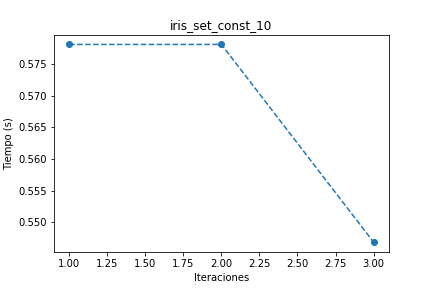
\includegraphics[width=0.234\textwidth]{img/copkm/iris_set_const_10_949004259_time.png}
    \end{subfigure}
    \hfill
    \begin{subfigure}
        \centering
        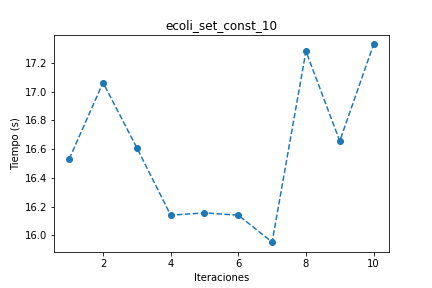
\includegraphics[width=0.234\textwidth]{img/copkm/ecoli_set_const_10_949004259_time.png}
    \end{subfigure}
    \hfill
    \begin{subfigure}
        \centering
        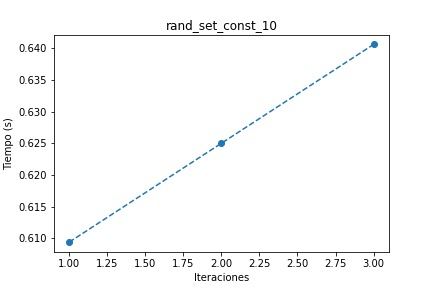
\includegraphics[width=0.234\textwidth]{img/copkm/rand_set_const_10_949004259_time.png}
    \end{subfigure}
    \hfill
    \begin{subfigure}
        \centering
        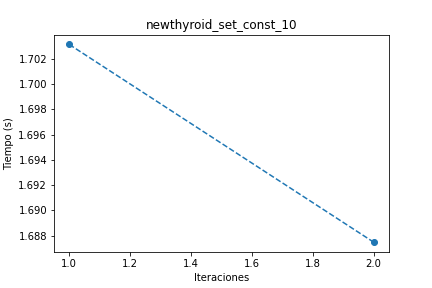
\includegraphics[width=0.234\textwidth]{img/copkm/newthyroid_set_const_10_949004259_time.png}
    \end{subfigure}
    \hfill
    \begin{subfigure}
        \centering
        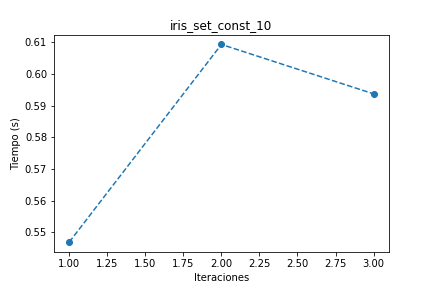
\includegraphics[width=0.234\textwidth]{img/copkm/iris_set_const_10_589741062_time.png}
    \end{subfigure}
    \hfill
    \begin{subfigure}
        \centering
        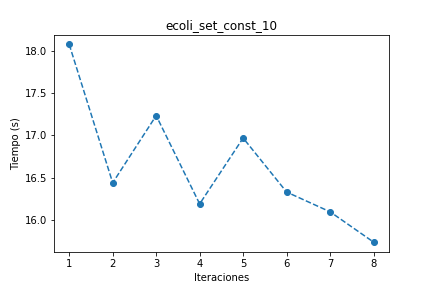
\includegraphics[width=0.234\textwidth]{img/copkm/ecoli_set_const_10_589741062_time.png}
    \end{subfigure}
    \hfill
    \begin{subfigure}
        \centering
        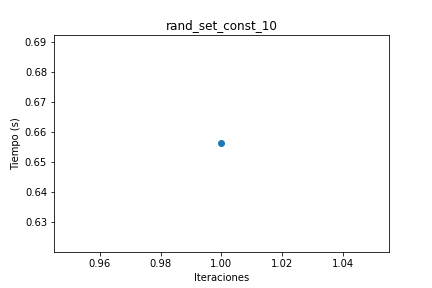
\includegraphics[width=0.234\textwidth]{img/copkm/rand_set_const_10_589741062_time.png}
    \end{subfigure}
    \hfill
    \begin{subfigure}
        \centering
        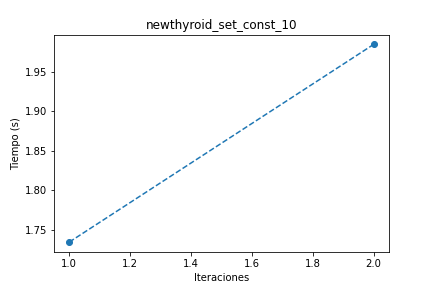
\includegraphics[width=0.234\textwidth]{img/copkm/newthyroid_set_const_10_589741062_time.png}
    \end{subfigure}
    \hfill
    \begin{subfigure}
        \centering
        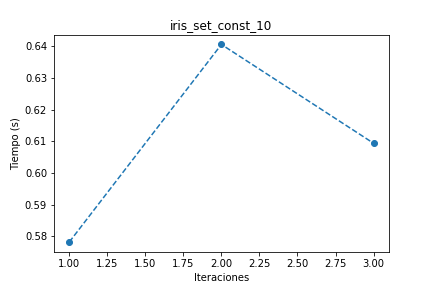
\includegraphics[width=0.234\textwidth]{img/copkm/iris_set_const_10_277451237_time.png}
    \end{subfigure}
    \hfill
    \begin{subfigure}
        \centering
        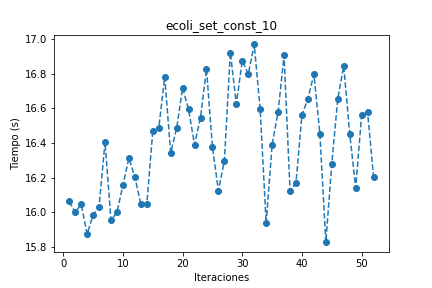
\includegraphics[width=0.234\textwidth]{img/copkm/ecoli_set_const_10_277451237_time.png}
    \end{subfigure}
    \hfill
    \begin{subfigure}
        \centering
        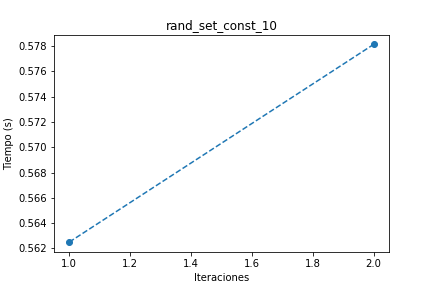
\includegraphics[width=0.234\textwidth]{img/copkm/rand_set_const_10_277451237_time.png}
    \end{subfigure}
    \hfill
    \begin{subfigure}
        \centering
        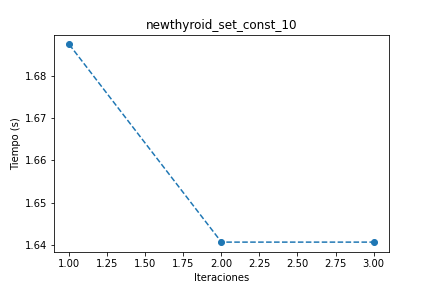
\includegraphics[width=0.234\textwidth]{img/copkm/newthyroid_set_const_10_277451237_time.png}
    \end{subfigure}
    \hfill
    \begin{subfigure}
        \centering
        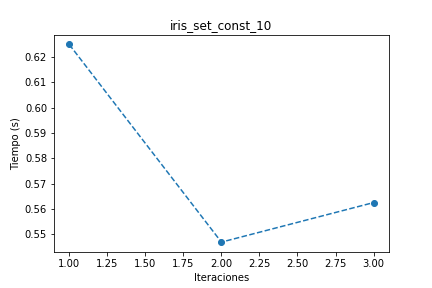
\includegraphics[width=0.234\textwidth]{img/copkm/iris_set_const_10_49258669_time.png}
    \end{subfigure}
    \hfill
    \begin{subfigure}
        \centering
        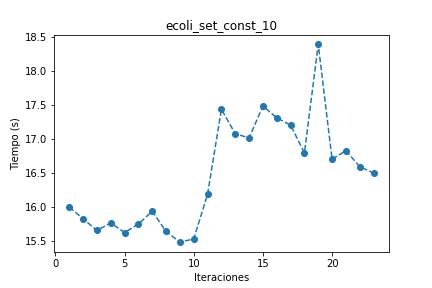
\includegraphics[width=0.234\textwidth]{img/copkm/ecoli_set_const_10_49258669_time.png}
    \end{subfigure}
    \hfill
    \begin{subfigure}
        \centering
        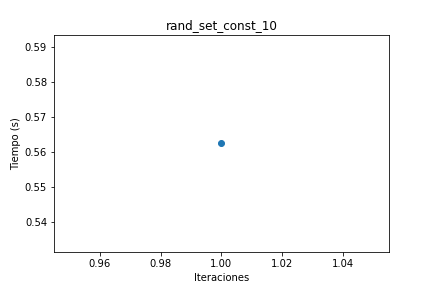
\includegraphics[width=0.234\textwidth]{img/copkm/rand_set_const_10_49258669_time.png}
    \end{subfigure}
    \hfill
    \begin{subfigure}
        \centering
        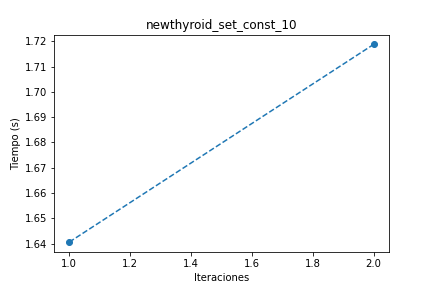
\includegraphics[width=0.234\textwidth]{img/copkm/newthyroid_set_const_10_49258669_time.png}
    \end{subfigure}
    \hfill
    \begin{subfigure}
        \centering
        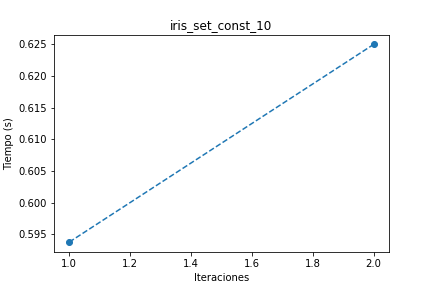
\includegraphics[width=0.234\textwidth]{img/copkm/iris_set_const_10_3773969821_time.png}
    \end{subfigure}
    \hfill
    \begin{subfigure}
        \centering
        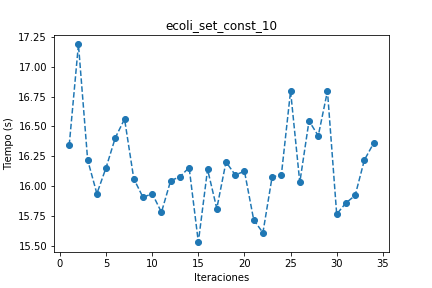
\includegraphics[width=0.234\textwidth]{img/copkm/ecoli_set_const_10_3773969821_time.png}
    \end{subfigure}
    \hfill
    \begin{subfigure}
        \centering
        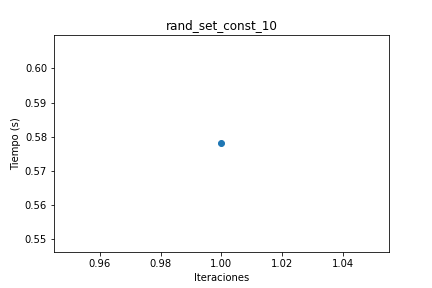
\includegraphics[width=0.234\textwidth]{img/copkm/rand_set_const_10_3773969821_time.png}
    \end{subfigure}
    \hfill
    \begin{subfigure}
        \centering
        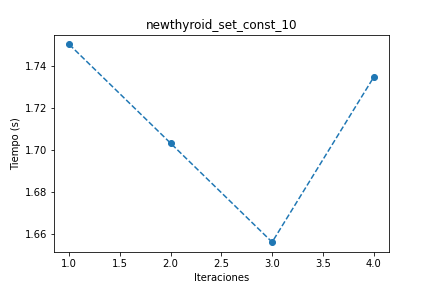
\includegraphics[width=0.234\textwidth]{img/copkm/newthyroid_set_const_10_3773969821_time.png}
    \end{subfigure}
    \caption{Tiempos de COPKM v1 para 10\% de restricciones}
\end{figure}

\vspace*{\fill}
\newpage
\vspace*{\fill}

\begin{figure}[H]
    \centering
    \begin{subfigure}
        \centering
        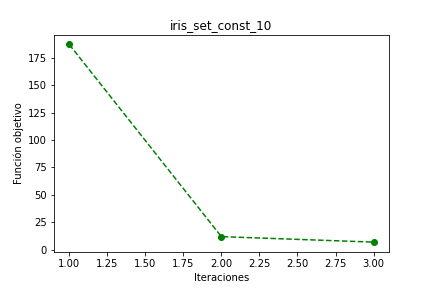
\includegraphics[width=0.234\textwidth]{img/copkm/iris_set_const_10_949004259_cost.png}
    \end{subfigure}
    \hfill
    \begin{subfigure}
        \centering
        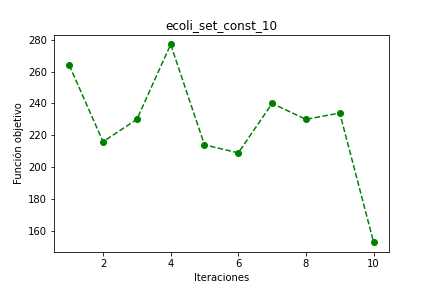
\includegraphics[width=0.234\textwidth]{img/copkm/ecoli_set_const_10_949004259_cost.png}
    \end{subfigure}
    \hfill
    \begin{subfigure}
        \centering
        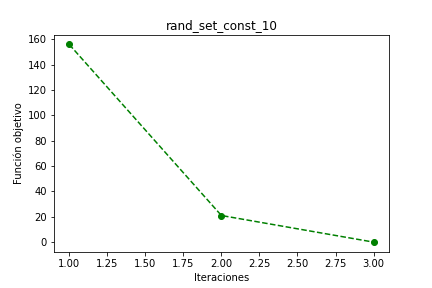
\includegraphics[width=0.234\textwidth]{img/copkm/rand_set_const_10_949004259_cost.png}
    \end{subfigure}
    \hfill
    \begin{subfigure}
        \centering
        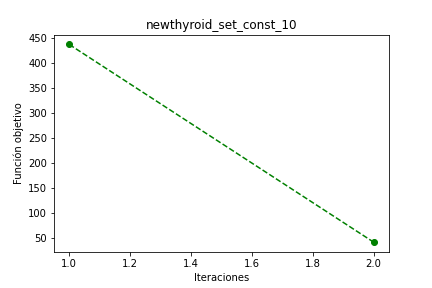
\includegraphics[width=0.234\textwidth]{img/copkm/newthyroid_set_const_10_949004259_cost.png}
    \end{subfigure}
    \hfill
    \begin{subfigure}
        \centering
        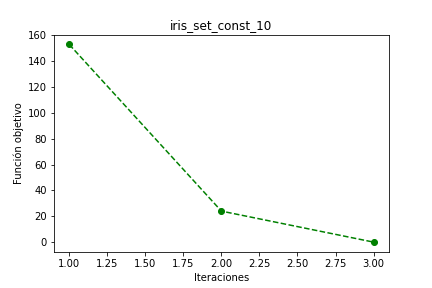
\includegraphics[width=0.234\textwidth]{img/copkm/iris_set_const_10_589741062_cost.png}
    \end{subfigure}
    \hfill
    \begin{subfigure}
        \centering
        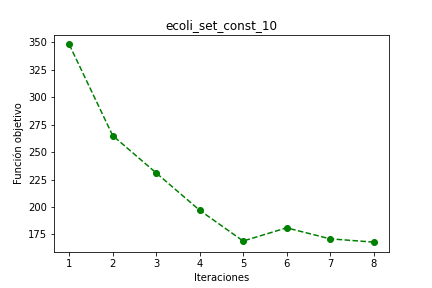
\includegraphics[width=0.234\textwidth]{img/copkm/ecoli_set_const_10_589741062_cost.png}
    \end{subfigure}
    \hfill
    \begin{subfigure}
        \centering
        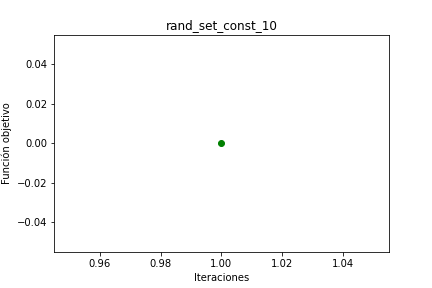
\includegraphics[width=0.234\textwidth]{img/copkm/rand_set_const_10_589741062_cost.png}
    \end{subfigure}
    \hfill
    \begin{subfigure}
        \centering
        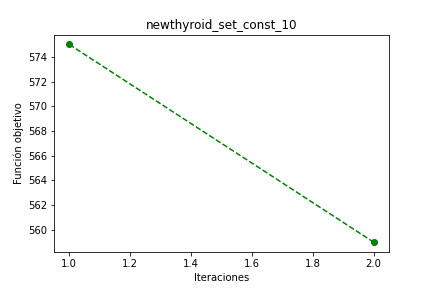
\includegraphics[width=0.234\textwidth]{img/copkm/newthyroid_set_const_10_589741062_cost.png}
    \end{subfigure}
    \hfill
    \begin{subfigure}
        \centering
        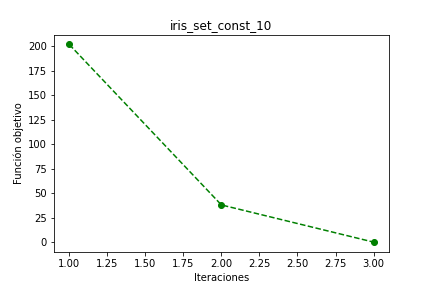
\includegraphics[width=0.234\textwidth]{img/copkm/iris_set_const_10_277451237_cost.png}
    \end{subfigure}
    \hfill
    \begin{subfigure}
        \centering
        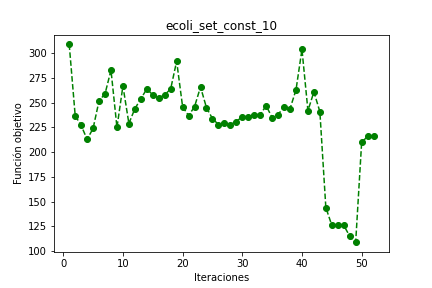
\includegraphics[width=0.234\textwidth]{img/copkm/ecoli_set_const_10_277451237_cost.png}
    \end{subfigure}
    \hfill
    \begin{subfigure}
        \centering
        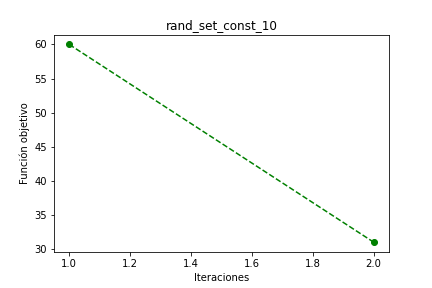
\includegraphics[width=0.234\textwidth]{img/copkm/rand_set_const_10_277451237_cost.png}
    \end{subfigure}
    \hfill
    \begin{subfigure}
        \centering
        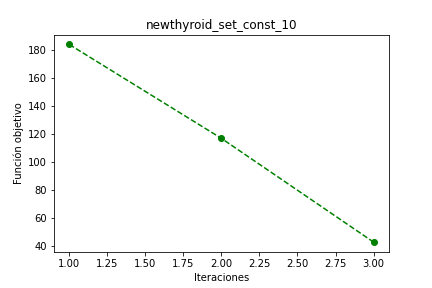
\includegraphics[width=0.234\textwidth]{img/copkm/newthyroid_set_const_10_277451237_cost.png}
    \end{subfigure}
    \hfill
    \begin{subfigure}
        \centering
        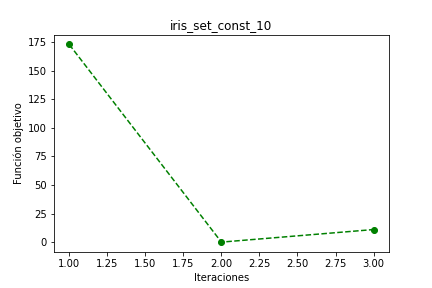
\includegraphics[width=0.234\textwidth]{img/copkm/iris_set_const_10_49258669_cost.png}
    \end{subfigure}
    \hfill
    \begin{subfigure}
        \centering
        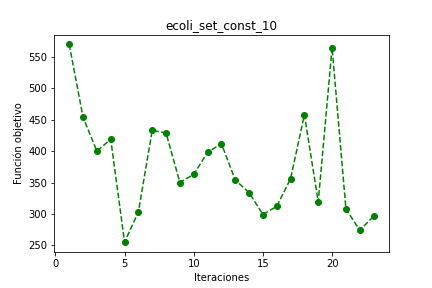
\includegraphics[width=0.234\textwidth]{img/copkm/ecoli_set_const_10_49258669_cost.png}
    \end{subfigure}
    \hfill
    \begin{subfigure}
        \centering
        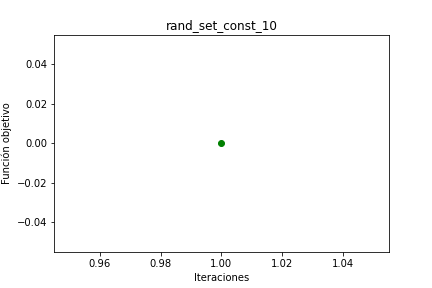
\includegraphics[width=0.234\textwidth]{img/copkm/rand_set_const_10_49258669_cost.png}
    \end{subfigure}
    \hfill
    \begin{subfigure}
        \centering
        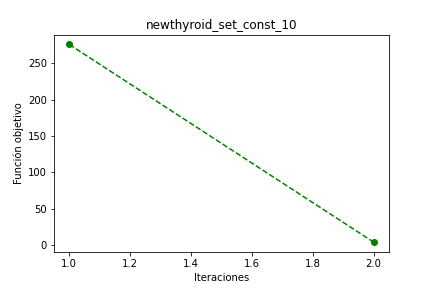
\includegraphics[width=0.234\textwidth]{img/copkm/newthyroid_set_const_10_49258669_cost.png}
    \end{subfigure}
    \hfill
    \begin{subfigure}
        \centering
        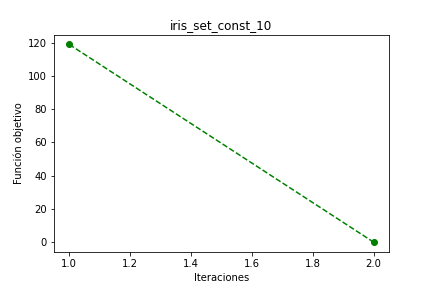
\includegraphics[width=0.234\textwidth]{img/copkm/iris_set_const_10_3773969821_cost.png}
    \end{subfigure}
    \hfill
    \begin{subfigure}
        \centering
        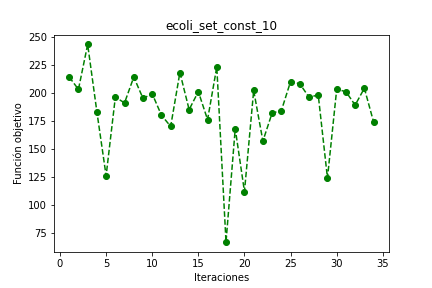
\includegraphics[width=0.234\textwidth]{img/copkm/ecoli_set_const_10_3773969821_cost.png}
    \end{subfigure}
    \hfill
    \begin{subfigure}
        \centering
        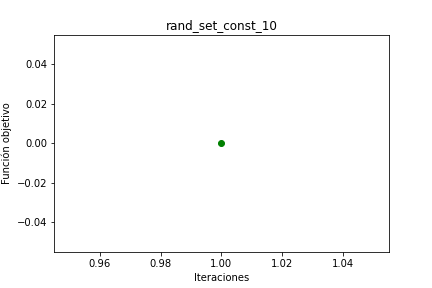
\includegraphics[width=0.234\textwidth]{img/copkm/rand_set_const_10_3773969821_cost.png}
    \end{subfigure}
    \hfill
    \begin{subfigure}
        \centering
        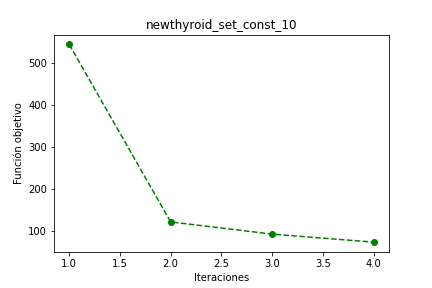
\includegraphics[width=0.234\textwidth]{img/copkm/newthyroid_set_const_10_3773969821_cost.png}
    \end{subfigure}
    \caption{Agregado de COPKM v1 para 10\% de restricciones}
\end{figure}

% ------------------------------------------------------------------------------

\vspace*{\fill}

\newpage

\vspace*{\fill}

\begin{table}[H]
    \centering
    \resizebox{0.85\columnwidth}{!}{%
    \makebox[\textwidth][c]{
        \begin{tabular}{|| c || c c c c || c c c c || c c c c || c c c c ||} 
            \hline
            & \multicolumn{4}{|c||}{Iris} & \multicolumn{4}{|c||}{Ecoli} & \multicolumn{4}{|c|}{Rand} & \multicolumn{4}{|c|}{Newthyroid}\\
            \hline
            & TasaC & TasaInf & Agr & T & TasaC & TasaInf & Agr & T & TasaC & TasaInf & Agr & T & TasaC & TasaInf & Agr & T \\
            \hline\hline
            Ejecución 1 & 0.67 & 17.00 & 0.72 & 3.36 & 34.44 & 351.00 & 39.15 & 169.77 & 0.76 & 0.00 & 0.76 & 3.38 
            & 14.20 & 67.00 & 15.42 & 10.00
            \\
            \hline
            Ejecución 2 & 0.67 & 0.00 & 0.67 & 2.33 & 37.64 & 158.00 & 39.76 & 283.50 & 0.76 & 0.00 & 0.76 & 2.19 
            & 14.13 & 30.00 & 14.68 & 9.89
            \\
            \hline
            Ejecución 3 & 0.67 & 0.00 & 0.67 & 5.56 & 33.53 & 128.00 & 35.25 & 366.92 & 0.83 & 68.00 & 1.08 & 3.28 
            & 14.23 & 60.00 & 15.33 & 9.83
            \\
            \hline
            Ejecución 4 & 0.67 & 0.00 & 0.67 & 3.22 & 32.35 & 92.00 & 33.58 & 392.08 & 0.76 & 0.00 & 0.76 & 2.31 
            & 14.23 & 30.00 & 14.78 & 13.19
            \\
            \hline
            Ejecución 5 & 0.67 & 0.00 & 0.67 & 3.30 & 37.46 & 118.00 & 39.04 & 158.39 & 0.76 & 0.00 & 0.76 & 2.14 
            & 14.13 & 14.13 & 15.39 & 9.81
            \\
            \hline\hline
            Media & 0.67 & 3.40 & 0.68 & 3.55 & 35.08 & 169.40 & 37.36 & 274.13 & 0.77 & 13.60 & 0.82 & 2.66 
            & 14.18 & 40.23 & 15.12 & 10.54
            \\
            \hline
        \end{tabular}
    }
    }
    \caption{Resultados COPKM v1 para 20\% de restricciones}
\end{table}

\vspace*{\fill}

\newpage

\vspace*{\fill}

\begin{figure}[H]    
    \centering
    \begin{subfigure}
        \centering
        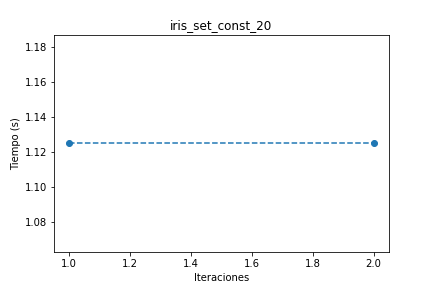
\includegraphics[width=0.234\textwidth]{img/copkm/iris_set_const_20_949004259_time.png}
    \end{subfigure}
    \hfill
    \begin{subfigure}
        \centering
        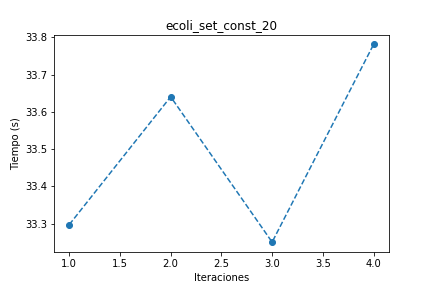
\includegraphics[width=0.234\textwidth]{img/copkm/ecoli_set_const_20_949004259_time.png}
    \end{subfigure}
    \hfill
    \begin{subfigure}
        \centering
        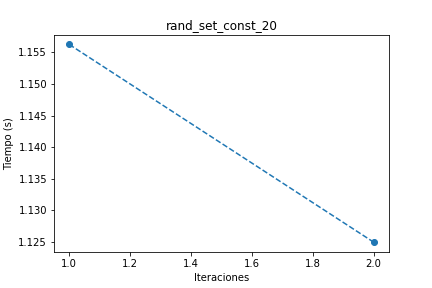
\includegraphics[width=0.234\textwidth]{img/copkm/rand_set_const_20_949004259_time.png}
    \end{subfigure}
    \hfill
    \begin{subfigure}
        \centering
        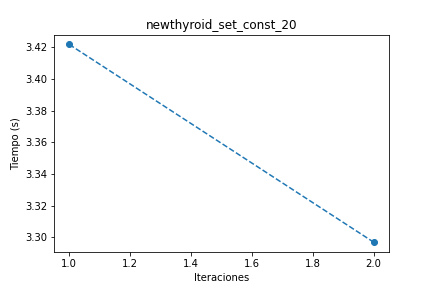
\includegraphics[width=0.234\textwidth]{img/copkm/newthyroid_set_const_20_949004259_time.png}
    \end{subfigure}
    \hfill
    \begin{subfigure}
        \centering
        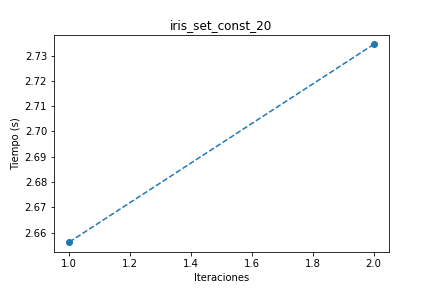
\includegraphics[width=0.234\textwidth]{img/copkm/iris_set_const_20_589741062_time.png}
    \end{subfigure}
    \hfill
    \begin{subfigure}
        \centering
        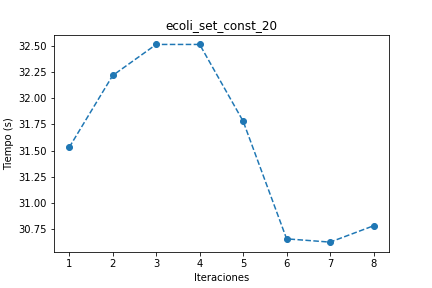
\includegraphics[width=0.234\textwidth]{img/copkm/ecoli_set_const_20_589741062_time.png}
    \end{subfigure}
    \hfill
    \begin{subfigure}
        \centering
        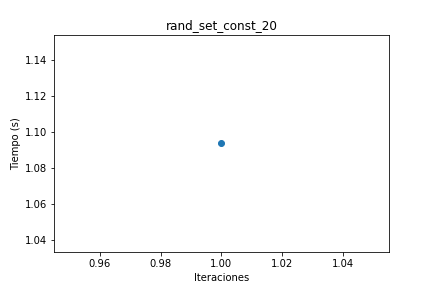
\includegraphics[width=0.234\textwidth]{img/copkm/rand_set_const_20_589741062_time.png}
    \end{subfigure}
    \hfill
    \begin{subfigure}
        \centering
        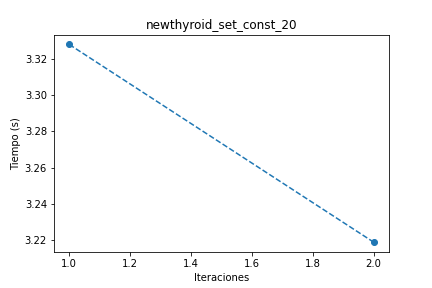
\includegraphics[width=0.234\textwidth]{img/copkm/newthyroid_set_const_20_589741062_time.png}
    \end{subfigure}
    \hfill
    \begin{subfigure}
        \centering
        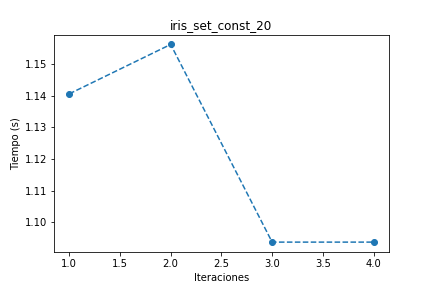
\includegraphics[width=0.234\textwidth]{img/copkm/iris_set_const_20_277451237_time.png}
    \end{subfigure}
    \hfill
    \begin{subfigure}
        \centering
        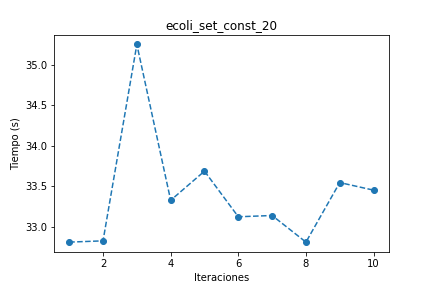
\includegraphics[width=0.234\textwidth]{img/copkm/ecoli_set_const_20_277451237_time.png}
    \end{subfigure}
    \hfill
    \begin{subfigure}
        \centering
        \includegraphics[width=0.234\textwidth]{img/copkm/rand_set_const_20_277451237_time.png}
    \end{subfigure}
    \hfill
    \begin{subfigure}
        \centering
        \includegraphics[width=0.234\textwidth]{img/copkm/newthyroid_set_const_20_277451237_time.png}
    \end{subfigure}
    \hfill
    \begin{subfigure}
        \centering
        \includegraphics[width=0.234\textwidth]{img/copkm/iris_set_const_20_49258669_time.png}
    \end{subfigure}
    \hfill
    \begin{subfigure}
        \centering
        \includegraphics[width=0.234\textwidth]{img/copkm/ecoli_set_const_20_49258669_time.png}
    \end{subfigure}
    \hfill
    \begin{subfigure}
        \centering
        \includegraphics[width=0.234\textwidth]{img/copkm/rand_set_const_20_49258669_time.png}
    \end{subfigure}
    \hfill
    \begin{subfigure}
        \centering
        \includegraphics[width=0.234\textwidth]{img/copkm/newthyroid_set_const_20_49258669_time.png}
    \end{subfigure}
    \hfill
    \begin{subfigure}
        \centering
        \includegraphics[width=0.234\textwidth]{img/copkm/iris_set_const_20_3773969821_time.png}
    \end{subfigure}
    \hfill
    \begin{subfigure}
        \centering
        \includegraphics[width=0.234\textwidth]{img/copkm/ecoli_set_const_20_3773969821_time.png}
    \end{subfigure}
    \hfill
    \begin{subfigure}
        \centering
        \includegraphics[width=0.234\textwidth]{img/copkm/rand_set_const_20_3773969821_time.png}
    \end{subfigure}
    \hfill
    \begin{subfigure}
        \centering
        \includegraphics[width=0.234\textwidth]{img/copkm/newthyroid_set_const_20_3773969821_time.png}
    \end{subfigure}
    \caption{Tiempos de COPKM v1 para 20\% de restricciones}
\end{figure}

\vspace*{\fill}

\newpage

\vspace*{\fill}

\begin{figure}[H]
    \centering
    \begin{subfigure}
        \centering
        \includegraphics[width=0.234\textwidth]{img/copkm/iris_set_const_20_949004259_cost.png}
    \end{subfigure}
    \hfill
    \begin{subfigure}
        \centering
        \includegraphics[width=0.234\textwidth]{img/copkm/ecoli_set_const_20_949004259_cost.png}
    \end{subfigure}
    \hfill
    \begin{subfigure}
        \centering
        \includegraphics[width=0.234\textwidth]{img/copkm/rand_set_const_20_949004259_cost.png}
    \end{subfigure}
    \hfill
    \begin{subfigure}
        \centering
        \includegraphics[width=0.234\textwidth]{img/copkm/newthyroid_set_const_20_949004259_cost.png}
    \end{subfigure}
    \hfill
    \begin{subfigure}
        \centering
        \includegraphics[width=0.234\textwidth]{img/copkm/iris_set_const_20_589741062_cost.png}
    \end{subfigure}
    \hfill
    \begin{subfigure}
        \centering
        \includegraphics[width=0.234\textwidth]{img/copkm/ecoli_set_const_20_589741062_cost.png}
    \end{subfigure}
    \hfill
    \begin{subfigure}
        \centering
        \includegraphics[width=0.234\textwidth]{img/copkm/rand_set_const_20_589741062_cost.png}
    \end{subfigure}
    \hfill
    \begin{subfigure}
        \centering
        \includegraphics[width=0.234\textwidth]{img/copkm/newthyroid_set_const_20_589741062_cost.png}
    \end{subfigure}
    \hfill
    \begin{subfigure}
        \centering
        \includegraphics[width=0.234\textwidth]{img/copkm/iris_set_const_20_277451237_cost.png}
    \end{subfigure}
    \hfill
    \begin{subfigure}
        \centering
        \includegraphics[width=0.234\textwidth]{img/copkm/ecoli_set_const_20_277451237_cost.png}
    \end{subfigure}
    \hfill
    \begin{subfigure}
        \centering
        \includegraphics[width=0.234\textwidth]{img/copkm/rand_set_const_20_277451237_cost.png}
    \end{subfigure}
    \hfill
    \begin{subfigure}
        \centering
        \includegraphics[width=0.234\textwidth]{img/copkm/newthyroid_set_const_20_277451237_cost.png}
    \end{subfigure}
    \hfill
    \begin{subfigure}
        \centering
        \includegraphics[width=0.234\textwidth]{img/copkm/iris_set_const_20_49258669_cost.png}
    \end{subfigure}
    \hfill
    \begin{subfigure}
        \centering
        \includegraphics[width=0.234\textwidth]{img/copkm/ecoli_set_const_20_49258669_cost.png}
    \end{subfigure}
    \hfill
    \begin{subfigure}
        \centering
        \includegraphics[width=0.234\textwidth]{img/copkm/rand_set_const_20_49258669_cost.png}
    \end{subfigure}
    \hfill
    \begin{subfigure}
        \centering
        \includegraphics[width=0.234\textwidth]{img/copkm/newthyroid_set_const_20_49258669_cost.png}
    \end{subfigure}
    \hfill
    \begin{subfigure}
        \centering
        \includegraphics[width=0.234\textwidth]{img/copkm/iris_set_const_20_3773969821_cost.png}
    \end{subfigure}
    \hfill
    \begin{subfigure}
        \centering
        \includegraphics[width=0.234\textwidth]{img/copkm/ecoli_set_const_20_3773969821_cost.png}
    \end{subfigure}
    \hfill
    \begin{subfigure}
        \centering
        \includegraphics[width=0.234\textwidth]{img/copkm/rand_set_const_20_3773969821_cost.png}
    \end{subfigure}
    \hfill
    \begin{subfigure}
        \centering
        \includegraphics[width=0.234\textwidth]{img/copkm/newthyroid_set_const_20_3773969821_cost.png}
    \end{subfigure}
    \caption{Agregado de COPKM v1 para 20\% de restricciones}
\end{figure}

\vspace*{\fill}

\newpage

\subsection{Búsqueda Local}

En todas las ejecuciones se utilizó un valor $\lambda$ igual al cociente entre la mayor distancia entre dos elementos cualesquiera del conjunto de datos y el número de restricciones del problema.

\begin{equation}    
    \lambda = \frac{\max D}{|R|}
\end{equation}

\vspace{\baselineskip}

% Gráfica con consume de tiempo por ciclo

\vspace*{\fill}

\begin{table}[H]
    \centering
    \resizebox{0.85\columnwidth}{!}{%
    \makebox[\textwidth][c]{
        \begin{tabular}{|| c || c c c c || c c c c || c c c c || c c c c ||} 
            \hline
            & \multicolumn{4}{|c||}{Iris} & \multicolumn{4}{|c||}{Ecoli} & \multicolumn{4}{|c|}{Rand} & \multicolumn{4}{|c|}{Newthyroid}\\
            \hline
            & TasaC & TasaInf & Agr & T & TasaC & TasaInf & Agr & T & TasaC & TasaInf & Agr & T & TasaC & TasaInf & Agr & T \\
            \hline\hline
            Ejecución 1 & 1.07 & 241.00 & 2.60 & 17.27 & 46.46 & 1188.00 & 78.34 & 747.25 & 1.22 & 131.00 & 2.17 & 27.70 
            & 14.87 & 271.00 & 24.78 & 157.25
            \\
            \hline
            Ejecución 2 & 1.02 & 193.00 & 2.24 & 20.77 & 46.63 & 1207.00 & 79.01 & 712.41 & 1.23 & 133.00 & 2.19 & 21.05 
            & 14.27 & 221.00 & 22.36 & 128.27
            \\
            \hline
            Ejecución 3 & 1.02 & 133.00 & 1.86 & 30.67 & 46.63 & 1228.00 & 79.58 & 741.86 & 1.14 & 133.00 & 2.10 & 35.20 
            & 14.40 & 388.00 & 28.59 & 122.80
            \\
            \hline
            Ejecución 4 & 0.76 & 75.00 & 1.23 & 29.66 & 47.39 & 1197.00 & 79.50 & 753.13 & 1.04 & 78.00 & 1.61 & 29.38 
            & 13.05 & 302.00 & 24.10 & 141.84
            \\
            \hline
            Ejecución 5 & 0.76 & 64.00 & 1.16 & 39.13 & 46.60 & 1244.00 & 79.98 & 712.03 & 0.95 & 55.00 & 1.35 & 32.73 
            & 14.22 & 302.00 & 25.27 & 110.33
            \\
            \hline\hline
            Media & 0.92 & 141.20 & 1.82 & 27.50 & 46.74 & 1212.80 & 79.28 & 733.33 & 1.12 & 106.00 & 1.88 & 29.21 
            & 14.16 & 296.80 & 25.02 & 132.10
            \\
            \hline
        \end{tabular}
    }
    }
    \caption{Resultados BL para 10\% de restricciones}
\end{table}

\vspace*{\fill}
\newpage
\vspace*{\fill}

\begin{figure}[H]
    \centering
    \begin{subfigure}
        \centering
        \includegraphics[width=0.234\textwidth]{img/bl/iris_set_const_10_949004259_time.png}
    \end{subfigure}
    \hfill
    \begin{subfigure}
        \centering
        \includegraphics[width=0.234\textwidth]{img/bl/ecoli_set_const_10_949004259_time.png}
    \end{subfigure}
    \hfill
    \begin{subfigure}
        \centering
        \includegraphics[width=0.234\textwidth]{img/bl/rand_set_const_10_949004259_time.png}
    \end{subfigure}
    \hfill
    \begin{subfigure}
        \centering
        \includegraphics[width=0.234\textwidth]{img/bl/newthyroid_set_const_10_949004259_time.png}
    \end{subfigure}
    \hfill
    \begin{subfigure}
        \centering
        \includegraphics[width=0.234\textwidth]{img/bl/iris_set_const_10_589741062_time.png}
    \end{subfigure}
    \hfill
    \begin{subfigure}
        \centering
        \includegraphics[width=0.234\textwidth]{img/bl/ecoli_set_const_10_589741062_time.png}
    \end{subfigure}
    \hfill
    \begin{subfigure}
        \centering
        \includegraphics[width=0.234\textwidth]{img/bl/rand_set_const_10_589741062_time.png}
    \end{subfigure}
    \hfill
    \begin{subfigure}
        \centering
        \includegraphics[width=0.234\textwidth]{img/bl/newthyroid_set_const_10_589741062_time.png}
    \end{subfigure}
    \hfill
    \begin{subfigure}
        \centering
        \includegraphics[width=0.234\textwidth]{img/bl/iris_set_const_10_277451237_time.png}
    \end{subfigure}
    \hfill
    \begin{subfigure}
        \centering
        \includegraphics[width=0.234\textwidth]{img/bl/ecoli_set_const_10_277451237_time.png}
    \end{subfigure}
    \hfill
    \begin{subfigure}
        \centering
        \includegraphics[width=0.234\textwidth]{img/bl/rand_set_const_10_277451237_time.png}
    \end{subfigure}
    \hfill
    \begin{subfigure}
        \centering
        \includegraphics[width=0.234\textwidth]{img/bl/newthyroid_set_const_10_277451237_time.png}
    \end{subfigure}
    \hfill
    \begin{subfigure}
        \centering
        \includegraphics[width=0.234\textwidth]{img/bl/iris_set_const_10_49258669_time.png}
    \end{subfigure}
    \hfill
    \begin{subfigure}
        \centering
        \includegraphics[width=0.234\textwidth]{img/bl/ecoli_set_const_10_49258669_time.png}
    \end{subfigure}
    \hfill
    \begin{subfigure}
        \centering
        \includegraphics[width=0.234\textwidth]{img/bl/rand_set_const_10_49258669_time.png}
    \end{subfigure}
    \hfill
    \begin{subfigure}
        \centering
        \includegraphics[width=0.234\textwidth]{img/bl/newthyroid_set_const_10_49258669_time.png}
    \end{subfigure}
    \hfill
    \begin{subfigure}
        \centering
        \includegraphics[width=0.234\textwidth]{img/bl/iris_set_const_10_3773969821_time.png}
    \end{subfigure}
    \hfill
    \begin{subfigure}
        \centering
        \includegraphics[width=0.234\textwidth]{img/bl/ecoli_set_const_10_3773969821_time.png}
    \end{subfigure}
    \hfill
    \begin{subfigure}
        \centering
        \includegraphics[width=0.234\textwidth]{img/bl/rand_set_const_10_3773969821_time.png}
    \end{subfigure}
    \hfill
    \begin{subfigure}
        \centering
        \includegraphics[width=0.234\textwidth]{img/bl/newthyroid_set_const_10_3773969821_time.png}
    \end{subfigure}
    \caption{Tiempos de BL para 10\% de restricciones}
\end{figure}

\vspace*{\fill}
\newpage
\vspace*{\fill}

\begin{figure}[H]
    \centering
    \begin{subfigure}
        \centering
        \includegraphics[width=0.234\textwidth]{img/bl/iris_set_const_10_949004259_cost.png}
    \end{subfigure}
    \hfill
    \begin{subfigure}
        \centering
        \includegraphics[width=0.234\textwidth]{img/bl/ecoli_set_const_10_949004259_cost.png}
    \end{subfigure}
    \hfill
    \begin{subfigure}
        \centering
        \includegraphics[width=0.234\textwidth]{img/bl/rand_set_const_10_949004259_cost.png}
    \end{subfigure}
    \hfill
    \begin{subfigure}
        \centering
        \includegraphics[width=0.234\textwidth]{img/bl/newthyroid_set_const_10_949004259_cost.png}
    \end{subfigure}
    \hfill
    \begin{subfigure}
        \centering
        \includegraphics[width=0.234\textwidth]{img/bl/iris_set_const_10_589741062_cost.png}
    \end{subfigure}
    \hfill
    \begin{subfigure}
        \centering
        \includegraphics[width=0.234\textwidth]{img/bl/ecoli_set_const_10_589741062_cost.png}
    \end{subfigure}
    \hfill
    \begin{subfigure}
        \centering
        \includegraphics[width=0.234\textwidth]{img/bl/rand_set_const_10_589741062_cost.png}
    \end{subfigure}
    \hfill
    \begin{subfigure}
        \centering
        \includegraphics[width=0.234\textwidth]{img/bl/newthyroid_set_const_10_589741062_cost.png}
    \end{subfigure}
    \hfill
    \begin{subfigure}
        \centering
        \includegraphics[width=0.234\textwidth]{img/bl/iris_set_const_10_277451237_cost.png}
    \end{subfigure}
    \hfill
    \begin{subfigure}
        \centering
        \includegraphics[width=0.234\textwidth]{img/bl/ecoli_set_const_10_277451237_cost.png}
    \end{subfigure}
    \hfill
    \begin{subfigure}
        \centering
        \includegraphics[width=0.234\textwidth]{img/bl/rand_set_const_10_277451237_cost.png}
    \end{subfigure}
    \hfill
    \begin{subfigure}
        \centering
        \includegraphics[width=0.234\textwidth]{img/bl/newthyroid_set_const_10_277451237_cost.png}
    \end{subfigure}
    \hfill
    \begin{subfigure}
        \centering
        \includegraphics[width=0.234\textwidth]{img/bl/iris_set_const_10_49258669_cost.png}
    \end{subfigure}
    \hfill
    \begin{subfigure}
        \centering
        \includegraphics[width=0.234\textwidth]{img/bl/ecoli_set_const_10_49258669_cost.png}
    \end{subfigure}
    \hfill
    \begin{subfigure}
        \centering
        \includegraphics[width=0.234\textwidth]{img/bl/rand_set_const_10_49258669_cost.png}
    \end{subfigure}
    \hfill
    \begin{subfigure}
        \centering
        \includegraphics[width=0.234\textwidth]{img/bl/newthyroid_set_const_10_49258669_cost.png}
    \end{subfigure}
    \hfill
    \begin{subfigure}
        \centering
        \includegraphics[width=0.234\textwidth]{img/bl/iris_set_const_10_3773969821_cost.png}
    \end{subfigure}
    \hfill
    \begin{subfigure}
        \centering
        \includegraphics[width=0.234\textwidth]{img/bl/ecoli_set_const_10_3773969821_cost.png}
    \end{subfigure}
    \hfill
    \begin{subfigure}
        \centering
        \includegraphics[width=0.234\textwidth]{img/bl/rand_set_const_10_3773969821_cost.png}
    \end{subfigure}
    \hfill
    \begin{subfigure}
        \centering
        \includegraphics[width=0.234\textwidth]{img/bl/newthyroid_set_const_10_3773969821_cost.png}
    \end{subfigure}
    \caption{Agregado de BL para 10\% de restricciones}
\end{figure}

\vspace*{\fill}
\newpage
\vspace*{\fill}

\begin{table}[H]
    \centering
    \resizebox{0.85\columnwidth}{!}{%
    \makebox[\textwidth][c]{
        \begin{tabular}{|| c || c c c c || c c c c || c c c c || c c c c ||} 
            \hline
            & \multicolumn{4}{|c||}{Iris} & \multicolumn{4}{|c||}{Ecoli} & \multicolumn{4}{|c|}{Rand} & \multicolumn{4}{|c|}{Newthyroid}\\
            \hline
            & TasaC & TasaInf & Agr & T & TasaC & TasaInf & Agr & T & TasaC & TasaInf & Agr & T & TasaC & TasaInf & Agr & T \\
            \hline\hline
            Ejecución 1 & 0.82 & 279.00 & 1.70 & 42.30 & 46.28 & 2133.00 & 74.89 & 1256.20 & 1.14 & 272.00 & 2.12 & 40.48 
            & 14.82 & 602.00 & 25.83 & 235.84
            \\
            \hline
            Ejecución 2 & 0.94 & 325.00 & 1.97 & 32.75 & 46.64 & 2194.00 & 76.07 & 1220.25 & 1.25 & 366.00 & 2.57 & 33.13 
            & 14.83 & 519.00 & 24.31 & 159.41
            \\
            \hline
            Ejecución 3 & 1.11 & 338.00 & 2.18 & 36.50 & 46.88 & 2178.00 & 76.10 & 1234.64 & 1.07 & 258.00 & 2.00 & 40.19 
            & 14.37 & 597.00 & 25.29 & 175.42
            \\
            \hline
            Ejecución 4 & 0.93 & 276.00 & 1.80 & 38.41 & 47.14 & 2190.00 & 76.52 & 1223.83 & 1.02 & 194.00 & 1.71 & 44.39 
            & 14.10 & 610.00 & 25.25 & 170.97
            \\
            \hline
            Ejecución 5 & 0.72 & 106.00 & 1.05 & 50.94 & 47.30 & 2181.00 & 76.56 & 1277.31 & 1.30 & 376.00 & 2.65 & 33.05  & 14.61 & 553.00 & 24.72 & 170.14
            \\
            \hline\hline
            Media & 0.90 & 264.80 & 1.74 & 40.18 & 46.85 & 2175.20 & 76.03 & 1242.45 & 1.15 & 293.20 & 2.21 & 38.25  & 14.54 & 576.20 & 25.08 & 182.36 \\
            \hline

        \end{tabular}
    }   
    }
    \caption{Resultados BL para 20\% de restricciones}
\end{table}

\vspace*{\fill}
\newpage
\vspace*{\fill}

\begin{figure}[H]    
    \centering
    \begin{subfigure}
        \centering
        \includegraphics[width=0.234\textwidth]{img/bl/iris_set_const_20_949004259_time.png}
    \end{subfigure}
    \hfill
    \begin{subfigure}
        \centering
        \includegraphics[width=0.234\textwidth]{img/bl/ecoli_set_const_20_949004259_time.png}
    \end{subfigure}
    \hfill
    \begin{subfigure}
        \centering
        \includegraphics[width=0.234\textwidth]{img/bl/rand_set_const_20_949004259_time.png}
    \end{subfigure}
    \hfill
    \begin{subfigure}
        \centering
        \includegraphics[width=0.234\textwidth]{img/bl/newthyroid_set_const_20_949004259_time.png}
    \end{subfigure}
    \hfill
    \begin{subfigure}
        \centering
        \includegraphics[width=0.234\textwidth]{img/bl/iris_set_const_20_589741062_time.png}
    \end{subfigure}
    \hfill
    \begin{subfigure}
        \centering
        \includegraphics[width=0.234\textwidth]{img/bl/ecoli_set_const_20_589741062_time.png}
    \end{subfigure}
    \hfill
    \begin{subfigure}
        \centering
        \includegraphics[width=0.234\textwidth]{img/bl/rand_set_const_20_589741062_time.png}
    \end{subfigure}
    \hfill
    \begin{subfigure}
        \centering
        \includegraphics[width=0.234\textwidth]{img/bl/newthyroid_set_const_20_589741062_time.png}
    \end{subfigure}
    \hfill
    \begin{subfigure}
        \centering
        \includegraphics[width=0.234\textwidth]{img/bl/iris_set_const_20_277451237_time.png}
    \end{subfigure}
    \hfill
    \begin{subfigure}
        \centering
        \includegraphics[width=0.234\textwidth]{img/bl/ecoli_set_const_20_277451237_time.png}
    \end{subfigure}
    \hfill
    \begin{subfigure}
        \centering
        \includegraphics[width=0.234\textwidth]{img/bl/rand_set_const_20_277451237_time.png}
    \end{subfigure}
    \hfill
    \begin{subfigure}
        \centering
        \includegraphics[width=0.234\textwidth]{img/bl/newthyroid_set_const_20_277451237_time.png}
    \end{subfigure}
    \hfill
    \begin{subfigure}
        \centering
        \includegraphics[width=0.234\textwidth]{img/bl/iris_set_const_20_49258669_time.png}
    \end{subfigure}
    \hfill
    \begin{subfigure}
        \centering
        \includegraphics[width=0.234\textwidth]{img/bl/ecoli_set_const_20_49258669_time.png}
    \end{subfigure}
    \hfill
    \begin{subfigure}
        \centering
        \includegraphics[width=0.234\textwidth]{img/bl/rand_set_const_20_49258669_time.png}
    \end{subfigure}
    \hfill
    \begin{subfigure}
        \centering
        \includegraphics[width=0.234\textwidth]{img/bl/newthyroid_set_const_20_49258669_time.png}
    \end{subfigure}
    \hfill
    \begin{subfigure}
        \centering
        \includegraphics[width=0.234\textwidth]{img/bl/iris_set_const_20_3773969821_time.png}
    \end{subfigure}
    \hfill
    \begin{subfigure}
        \centering
        \includegraphics[width=0.234\textwidth]{img/bl/ecoli_set_const_20_3773969821_time.png}
    \end{subfigure}
    \hfill
    \begin{subfigure}
        \centering
        \includegraphics[width=0.234\textwidth]{img/bl/rand_set_const_20_3773969821_time.png}
    \end{subfigure}
    \hfill
    \begin{subfigure}
        \centering
        \includegraphics[width=0.234\textwidth]{img/bl/newthyroid_set_const_20_3773969821_time.png}
    \end{subfigure}
    \caption{Tiempos de BL para 20\% de restricciones}
\end{figure}

\vspace*{\fill}
\newpage
\vspace*{\fill}

\begin{figure}[H]
    \centering
    \begin{subfigure}
        \centering
        \includegraphics[width=0.234\textwidth]{img/bl/iris_set_const_20_949004259_cost.png}
    \end{subfigure}
    \hfill
    \begin{subfigure}
        \centering
        \includegraphics[width=0.234\textwidth]{img/bl/ecoli_set_const_20_949004259_cost.png}
    \end{subfigure}
    \hfill
    \begin{subfigure}
        \centering
        \includegraphics[width=0.234\textwidth]{img/bl/rand_set_const_20_949004259_cost.png}
    \end{subfigure}
    \hfill
    \begin{subfigure}
        \centering
        \includegraphics[width=0.234\textwidth]{img/bl/newthyroid_set_const_20_949004259_cost.png}
    \end{subfigure}
    \hfill
    \begin{subfigure}
        \centering
        \includegraphics[width=0.234\textwidth]{img/bl/iris_set_const_20_589741062_cost.png}
    \end{subfigure}
    \hfill
    \begin{subfigure}
        \centering
        \includegraphics[width=0.234\textwidth]{img/bl/ecoli_set_const_20_589741062_cost.png}
    \end{subfigure}
    \hfill
    \begin{subfigure}
        \centering
        \includegraphics[width=0.234\textwidth]{img/bl/rand_set_const_20_589741062_cost.png}
    \end{subfigure}
    \hfill
    \begin{subfigure}
        \centering
        \includegraphics[width=0.234\textwidth]{img/bl/newthyroid_set_const_20_589741062_cost.png}
    \end{subfigure}
    \hfill
    \begin{subfigure}
        \centering
        \includegraphics[width=0.234\textwidth]{img/bl/iris_set_const_20_277451237_cost.png}
    \end{subfigure}
    \hfill
    \begin{subfigure}
        \centering
        \includegraphics[width=0.234\textwidth]{img/bl/ecoli_set_const_20_277451237_cost.png}
    \end{subfigure}
    \hfill
    \begin{subfigure}
        \centering
        \includegraphics[width=0.234\textwidth]{img/bl/rand_set_const_20_277451237_cost.png}
    \end{subfigure}
    \hfill
    \begin{subfigure}
        \centering
        \includegraphics[width=0.234\textwidth]{img/bl/newthyroid_set_const_20_277451237_cost.png}
    \end{subfigure}
    \hfill
    \begin{subfigure}
        \centering
        \includegraphics[width=0.234\textwidth]{img/bl/iris_set_const_20_49258669_cost.png}
    \end{subfigure}
    \hfill
    \begin{subfigure}
        \centering
        \includegraphics[width=0.234\textwidth]{img/bl/ecoli_set_const_20_49258669_cost.png}
    \end{subfigure}
    \hfill
    \begin{subfigure}
        \centering
        \includegraphics[width=0.234\textwidth]{img/bl/rand_set_const_20_49258669_cost.png}
    \end{subfigure}
    \hfill
    \begin{subfigure}
        \centering
        \includegraphics[width=0.234\textwidth]{img/bl/newthyroid_set_const_20_49258669_cost.png}
    \end{subfigure}
    \hfill
    \begin{subfigure}
        \centering
        \includegraphics[width=0.234\textwidth]{img/bl/iris_set_const_20_3773969821_cost.png}
    \end{subfigure}
    \hfill
    \begin{subfigure}
        \centering
        \includegraphics[width=0.234\textwidth]{img/bl/ecoli_set_const_20_3773969821_cost.png}
    \end{subfigure}
    \hfill
    \begin{subfigure}
        \centering
        \includegraphics[width=0.234\textwidth]{img/bl/rand_set_const_20_3773969821_cost.png}
    \end{subfigure}
    \hfill
    \begin{subfigure}
        \centering
        \includegraphics[width=0.234\textwidth]{img/bl/newthyroid_set_const_20_3773969821_cost.png}
    \end{subfigure}
    \caption{Agregado de BL para 20\% de restricciones}
\end{figure}

\vspace*{\fill}
\newpage

\subsection{Greedy COPKM v2}

\vspace*{\fill}

\begin{table}[H]
    \centering
    \resizebox{0.85\columnwidth}{!}{%
    \makebox[\textwidth][c]{
        \begin{tabular}{|| c || c c c c || c c c c || c c c c || c c c c ||} 
            \hline
            & \multicolumn{4}{|c||}{Iris} & \multicolumn{4}{|c||}{Ecoli} & \multicolumn{4}{|c|}{Rand} & \multicolumn{4}{|c|}{Newthyroid}\\
            \hline
            & TasaC & TasaInf & Agr & T & TasaC & TasaInf & Agr & T & TasaC & TasaInf & Agr & T & TasaC & TasaInf & Agr & T \\
            \hline\hline
            Ejecución 1 & 0.67 & 0.00 & 0.67 & 2.11 & 34.74 & 2.00 & 34.80 & 89.83 & 0.76 & 0.00 & 0.76 & 2.25 & 14.29 & 0.00 & 14.29 & 6.23 \\
            \hline
            Ejecución 2 & 0.67 & 0.00 & 0.67 & 2.72 & 29.37 & 0.00 & 29.37 & 152.09 & 0.76 & 0.00 & 0.76 & 1.66 & 14.29 & 0.00 & 14.29 & 6.39\\
            \hline
            Ejecución 3 & 0.67 & 0.00 & 0.67 & 2.89 & 57.53 & 277.00 & 64.96 & 59.25 & 0.76 & 0.00 & 0.76 & 2.27 & 14.29 & 0.00 & 14.29 & 8.56\\
            \hline
            Ejecución 4 & 0.67 & 0.00 & 0.67 & 2.22 & 33.71 & 4.00 & 33.71 & 106.02 & 0.76 & 0.00 & 0.76 & 1.69  & 14.29 & 0.00 & 14.29 & 6.97\\
            \hline
            Ejecución 5 & 0.67 & 0.00 & 0.67 & 2.25 & 32.15 & 3.00 & 32.23 & 182.00 & 0.76 & 0.00 & 0.76 & 2.25 & 14.29 & 0.00 & 14.29 & 6.22\\
            \hline\hline
            Media & 0.67 & 0.00 & 0.67 & 2.44 & 37.50 & 57.20 & 39.01 & 117.84 & 0.76 & 0.00 & 0.76 & 2.02 & 14.29 & 0.00 & 14.29 & 6.88 \\
            \hline

        \end{tabular}
    }
    }
    \caption{Resultados de COPKM v2 para 10\% de restricciones}
\end{table}

\vspace*{\fill}
\newpage
\vspace*{\fill}

\begin{figure}[H]    
    \centering
    \begin{subfigure}
        \centering
        \includegraphics[width=0.234\textwidth]{img/copkm2/iris_set_const_10_949004259_time.png}
    \end{subfigure}
    \hfill
    \begin{subfigure}
        \centering
        \includegraphics[width=0.234\textwidth]{img/copkm2/ecoli_set_const_10_949004259_time.png}
    \end{subfigure}
    \hfill
    \begin{subfigure}
        \centering
        \includegraphics[width=0.234\textwidth]{img/copkm2/rand_set_const_10_949004259_time.png}
    \end{subfigure}
    \hfill
    \begin{subfigure}
        \centering
        \includegraphics[width=0.234\textwidth]{img/copkm2/newthyroid_set_const_10_949004259_time.png}
    \end{subfigure}
    \hfill
    \begin{subfigure}
        \centering
        \includegraphics[width=0.234\textwidth]{img/copkm2/iris_set_const_10_589741062_time.png}
    \end{subfigure}
    \hfill
    \begin{subfigure}
        \centering
        \includegraphics[width=0.234\textwidth]{img/copkm2/ecoli_set_const_10_589741062_time.png}
    \end{subfigure}
    \hfill
    \begin{subfigure}
        \centering
        \includegraphics[width=0.234\textwidth]{img/copkm2/rand_set_const_10_589741062_time.png}
    \end{subfigure}
    \hfill
    \begin{subfigure}
        \centering
        \includegraphics[width=0.234\textwidth]{img/copkm2/newthyroid_set_const_10_589741062_time.png}
    \end{subfigure}
    \hfill
    \begin{subfigure}
        \centering
        \includegraphics[width=0.234\textwidth]{img/copkm2/iris_set_const_10_277451237_time.png}
    \end{subfigure}
    \hfill
    \begin{subfigure}
        \centering
        \includegraphics[width=0.234\textwidth]{img/copkm2/ecoli_set_const_10_277451237_time.png}
    \end{subfigure}
    \hfill
    \begin{subfigure}
        \centering
        \includegraphics[width=0.234\textwidth]{img/copkm2/rand_set_const_10_277451237_time.png}
    \end{subfigure}
    \hfill
    \begin{subfigure}
        \centering
        \includegraphics[width=0.234\textwidth]{img/copkm2/newthyroid_set_const_10_277451237_time.png}
    \end{subfigure}
    \hfill
    \begin{subfigure}
        \centering
        \includegraphics[width=0.234\textwidth]{img/copkm2/iris_set_const_10_49258669_time.png}
    \end{subfigure}
    \hfill
    \begin{subfigure}
        \centering
        \includegraphics[width=0.234\textwidth]{img/copkm2/ecoli_set_const_10_49258669_time.png}
    \end{subfigure}
    \hfill
    \begin{subfigure}
        \centering
        \includegraphics[width=0.234\textwidth]{img/copkm2/rand_set_const_10_49258669_time.png}
    \end{subfigure}
    \hfill
    \begin{subfigure}
        \centering
        \includegraphics[width=0.234\textwidth]{img/copkm2/newthyroid_set_const_10_49258669_time.png}
    \end{subfigure}
    \hfill
    \begin{subfigure}
        \centering
        \includegraphics[width=0.234\textwidth]{img/copkm2/iris_set_const_10_3773969821_time.png}
    \end{subfigure}
    \hfill
    \begin{subfigure}
        \centering
        \includegraphics[width=0.234\textwidth]{img/copkm2/ecoli_set_const_10_3773969821_time.png}
    \end{subfigure}
    \hfill
    \begin{subfigure}
        \centering
        \includegraphics[width=0.234\textwidth]{img/copkm2/rand_set_const_10_3773969821_time.png}
    \end{subfigure}
    \hfill
    \begin{subfigure}
        \centering
        \includegraphics[width=0.234\textwidth]{img/copkm2/newthyroid_set_const_10_3773969821_time.png}
    \end{subfigure}
    \caption{Tiempos de COPKM v2 para 10\% de restricciones}
\end{figure}

\vspace*{\fill}
\newpage
\vspace*{\fill}

\begin{figure}[H]
    \centering
    \begin{subfigure}
        \centering
        \includegraphics[width=0.234\textwidth]{img/copkm2/iris_set_const_10_949004259_cost.png}
    \end{subfigure}
    \hfill
    \begin{subfigure}
        \centering
        \includegraphics[width=0.234\textwidth]{img/copkm2/ecoli_set_const_10_949004259_cost.png}
    \end{subfigure}
    \hfill
    \begin{subfigure}
        \centering
        \includegraphics[width=0.234\textwidth]{img/copkm2/rand_set_const_10_949004259_cost.png}
    \end{subfigure}
    \hfill
    \begin{subfigure}
        \centering
        \includegraphics[width=0.234\textwidth]{img/copkm2/newthyroid_set_const_10_949004259_cost.png}
    \end{subfigure}
    \hfill
    \begin{subfigure}
        \centering
        \includegraphics[width=0.234\textwidth]{img/copkm2/iris_set_const_10_589741062_cost.png}
    \end{subfigure}
    \hfill
    \begin{subfigure}
        \centering
        \includegraphics[width=0.234\textwidth]{img/copkm2/ecoli_set_const_10_589741062_cost.png}
    \end{subfigure}
    \hfill
    \begin{subfigure}
        \centering
        \includegraphics[width=0.234\textwidth]{img/copkm2/rand_set_const_10_589741062_cost.png}
    \end{subfigure}
    \hfill
    \begin{subfigure}
        \centering
        \includegraphics[width=0.234\textwidth]{img/copkm2/newthyroid_set_const_10_589741062_cost.png}
    \end{subfigure}
    \hfill
    \begin{subfigure}
        \centering
        \includegraphics[width=0.234\textwidth]{img/copkm2/iris_set_const_10_277451237_cost.png}
    \end{subfigure}
    \hfill
    \begin{subfigure}
        \centering
        \includegraphics[width=0.234\textwidth]{img/copkm2/ecoli_set_const_10_277451237_cost.png}
    \end{subfigure}
    \hfill
    \begin{subfigure}
        \centering
        \includegraphics[width=0.234\textwidth]{img/copkm2/rand_set_const_10_277451237_cost.png}
    \end{subfigure}
    \hfill
    \begin{subfigure}
        \centering
        \includegraphics[width=0.234\textwidth]{img/copkm2/newthyroid_set_const_10_277451237_cost.png}
    \end{subfigure}
    \hfill
    \begin{subfigure}
        \centering
        \includegraphics[width=0.234\textwidth]{img/copkm2/iris_set_const_10_49258669_cost.png}
    \end{subfigure}
    \hfill
    \begin{subfigure}
        \centering
        \includegraphics[width=0.234\textwidth]{img/copkm2/ecoli_set_const_10_49258669_cost.png}
    \end{subfigure}
    \hfill
    \begin{subfigure}
        \centering
        \includegraphics[width=0.234\textwidth]{img/copkm2/rand_set_const_10_49258669_cost.png}
    \end{subfigure}
    \hfill
    \begin{subfigure}
        \centering
        \includegraphics[width=0.234\textwidth]{img/copkm2/newthyroid_set_const_10_49258669_cost.png}
    \end{subfigure}
    \hfill
    \begin{subfigure}
        \centering
        \includegraphics[width=0.234\textwidth]{img/copkm2/iris_set_const_10_3773969821_cost.png}
    \end{subfigure}
    \hfill
    \begin{subfigure}
        \centering
        \includegraphics[width=0.234\textwidth]{img/copkm2/ecoli_set_const_10_3773969821_cost.png}
    \end{subfigure}
    \hfill
    \begin{subfigure}
        \centering
        \includegraphics[width=0.234\textwidth]{img/copkm2/rand_set_const_10_3773969821_cost.png}
    \end{subfigure}
    \hfill
    \begin{subfigure}
        \centering
        \includegraphics[width=0.234\textwidth]{img/copkm2/newthyroid_set_const_10_3773969821_cost.png}
    \end{subfigure}
    \caption{Agregado de COPKM v2 para 10\% de restricciones}
\end{figure}

% ------------------------------------------------------------------------------

\vspace*{\fill}
\newpage
\vspace*{\fill}

\begin{table}[H]
    \centering
    \resizebox{0.85\columnwidth}{!}{%
    \makebox[\textwidth][c]{
        \begin{tabular}{|| c || c c c c || c c c c || c c c c || c c c c ||} 
            \hline
            & \multicolumn{4}{|c||}{Iris} & \multicolumn{4}{|c||}{Ecoli} & \multicolumn{4}{|c|}{Rand} & \multicolumn{4}{|c|}{Newthyroid}\\
            \hline
            & TasaC & TasaInf & Agr & T & TasaC & TasaInf & Agr & T & TasaC & TasaInf & Agr & T & TasaC & TasaInf & Agr & T \\
            \hline\hline
            Ejecución 1 & 0.67 & 0.00 & 0.67 & 3.25 & 29.61 & 0.00 & 29.61 & 183.00 & 0.76 & 0.00 & 0.76 & 3.19 & 14.29 & 0.00 & 14.29 & 14.91 \\
            \hline
            Ejecución 2 & 0.67 & 0.00 & 0.67 & 4.42 & 33.46 & 0.00 & 33.46 & 149.48 & 0.76 & 0.00 & 0.76 & 3.34 & 14.29 & 0.00 & 14.29 & 12.33 \\
            \hline
            Ejecución 3 & 0.67 & 0.00 & 0.67 & 4.33 & 34.43 & 0.00 & 34.43 & 93.83 & 0.76 & 0.00 & 0.76 & 3.30 & 14.29 & 0.00 & 14.29 & 9.36 \\
            \hline
            Ejecución 4 & 0.67 & 0.00 & 0.67 & 3.17 & 29.61 & 0.00 & 29.61 & 149.45 & 0.76 & 0.00 & 0.76 & 3.34 & 14.29 & 0.00 & 14.29 & 11.91 \\
            \hline
            Ejecución 5 & 0.67 & 0.00 & 0.67 & 3.27 & 28.40 & 0.00 & 28.40 & 150.48 & 0.76 & 0.00 & 0.76 & 3.14 & 14.29 & 0.00 & 14.29 & 12.14 \\
            \hline\hline
            Media & 0.67 & 0.00 & 0.67 & 3.69 & 31.10 & 0.00 & 31.10 & 145.25 & 0.76 & 0.00 & 0.76 & 3.26 & 14.29 & 0.00 & 14.29 & 12.13 \\
            \hline
        \end{tabular}
    }
    }
    \caption{Resultados de COPKM v2 para 20\% de restricciones}
\end{table}

\vspace*{\fill}
\newpage
\vspace*{\fill}

\begin{figure}[H]    
    \centering
    \begin{subfigure}
        \centering
        \includegraphics[width=0.234\textwidth]{img/copkm2/iris_set_const_20_949004259_time.png}
    \end{subfigure}
    \hfill
    \begin{subfigure}
        \centering
        \includegraphics[width=0.234\textwidth]{img/copkm2/ecoli_set_const_20_949004259_time.png}
    \end{subfigure}
    \hfill
    \begin{subfigure}
        \centering
        \includegraphics[width=0.234\textwidth]{img/copkm2/rand_set_const_20_949004259_time.png}
    \end{subfigure}
    \hfill
    \begin{subfigure}
        \centering
        \includegraphics[width=0.234\textwidth]{img/copkm2/newthyroid_set_const_20_949004259_time.png}
    \end{subfigure}
    \hfill
    \begin{subfigure}
        \centering
        \includegraphics[width=0.234\textwidth]{img/copkm2/iris_set_const_20_589741062_time.png}
    \end{subfigure}
    \hfill
    \begin{subfigure}
        \centering
        \includegraphics[width=0.234\textwidth]{img/copkm2/ecoli_set_const_20_589741062_time.png}
    \end{subfigure}
    \hfill
    \begin{subfigure}
        \centering
        \includegraphics[width=0.234\textwidth]{img/copkm2/rand_set_const_20_589741062_time.png}
    \end{subfigure}
    \hfill
    \begin{subfigure}
        \centering
        \includegraphics[width=0.234\textwidth]{img/copkm2/newthyroid_set_const_20_589741062_time.png}
    \end{subfigure}
    \hfill
    \begin{subfigure}
        \centering
        \includegraphics[width=0.234\textwidth]{img/copkm2/iris_set_const_20_277451237_time.png}
    \end{subfigure}
    \hfill
    \begin{subfigure}
        \centering
        \includegraphics[width=0.234\textwidth]{img/copkm2/ecoli_set_const_20_277451237_time.png}
    \end{subfigure}
    \hfill
    \begin{subfigure}
        \centering
        \includegraphics[width=0.234\textwidth]{img/copkm2/rand_set_const_20_277451237_time.png}
    \end{subfigure}
    \hfill
    \begin{subfigure}
        \centering
        \includegraphics[width=0.234\textwidth]{img/copkm2/newthyroid_set_const_20_277451237_time.png}
    \end{subfigure}
    \hfill
    \begin{subfigure}
        \centering
        \includegraphics[width=0.234\textwidth]{img/copkm2/iris_set_const_20_49258669_time.png}
    \end{subfigure}
    \hfill
    \begin{subfigure}
        \centering
        \includegraphics[width=0.234\textwidth]{img/copkm2/ecoli_set_const_20_49258669_time.png}
    \end{subfigure}
    \hfill
    \begin{subfigure}
        \centering
        \includegraphics[width=0.234\textwidth]{img/copkm2/rand_set_const_20_49258669_time.png}
    \end{subfigure}
    \hfill
    \begin{subfigure}
        \centering
        \includegraphics[width=0.234\textwidth]{img/copkm2/newthyroid_set_const_20_49258669_time.png}
    \end{subfigure}
    \hfill
    \begin{subfigure}
        \centering
        \includegraphics[width=0.234\textwidth]{img/copkm2/iris_set_const_20_3773969821_time.png}
    \end{subfigure}
    \hfill
    \begin{subfigure}
        \centering
        \includegraphics[width=0.234\textwidth]{img/copkm2/ecoli_set_const_20_3773969821_time.png}
    \end{subfigure}
    \hfill
    \begin{subfigure}
        \centering
        \includegraphics[width=0.234\textwidth]{img/copkm2/rand_set_const_20_3773969821_time.png}
    \end{subfigure}
    \hfill
    \begin{subfigure}
        \centering
        \includegraphics[width=0.234\textwidth]{img/copkm2/newthyroid_set_const_20_3773969821_time.png}
    \end{subfigure}
    \caption{Tiempos de COPKM v2 para 20\% de restricciones}
\end{figure}

\vspace*{\fill}
\newpage
\vspace*{\fill}

\begin{figure}[H]
    \centering
    \begin{subfigure}
        \centering
        \includegraphics[width=0.234\textwidth]{img/copkm2/iris_set_const_20_949004259_cost.png}
    \end{subfigure}
    \hfill
    \begin{subfigure}
        \centering
        \includegraphics[width=0.234\textwidth]{img/copkm2/ecoli_set_const_20_949004259_cost.png}
    \end{subfigure}
    \hfill
    \begin{subfigure}
        \centering
        \includegraphics[width=0.234\textwidth]{img/copkm2/rand_set_const_20_949004259_cost.png}
    \end{subfigure}
    \hfill
    \begin{subfigure}
        \centering
        \includegraphics[width=0.234\textwidth]{img/copkm2/newthyroid_set_const_20_949004259_cost.png}
    \end{subfigure}
    \hfill
    \begin{subfigure}
        \centering
        \includegraphics[width=0.234\textwidth]{img/copkm2/iris_set_const_20_589741062_cost.png}
    \end{subfigure}
    \hfill
    \begin{subfigure}
        \centering
        \includegraphics[width=0.234\textwidth]{img/copkm2/ecoli_set_const_20_589741062_cost.png}
    \end{subfigure}
    \hfill
    \begin{subfigure}
        \centering
        \includegraphics[width=0.234\textwidth]{img/copkm2/rand_set_const_20_589741062_cost.png}
    \end{subfigure}
    \hfill
    \begin{subfigure}
        \centering
        \includegraphics[width=0.234\textwidth]{img/copkm2/newthyroid_set_const_20_589741062_cost.png}
    \end{subfigure}
    \hfill
    \begin{subfigure}
        \centering
        \includegraphics[width=0.234\textwidth]{img/copkm2/iris_set_const_20_277451237_cost.png}
    \end{subfigure}
    \hfill
    \begin{subfigure}
        \centering
        \includegraphics[width=0.234\textwidth]{img/copkm2/ecoli_set_const_20_277451237_cost.png}
    \end{subfigure}
    \hfill
    \begin{subfigure}
        \centering
        \includegraphics[width=0.234\textwidth]{img/copkm2/rand_set_const_20_277451237_cost.png}
    \end{subfigure}
    \hfill
    \begin{subfigure}
        \centering
        \includegraphics[width=0.234\textwidth]{img/copkm2/newthyroid_set_const_20_277451237_cost.png}
    \end{subfigure}
    \hfill
    \begin{subfigure}
        \centering
        \includegraphics[width=0.234\textwidth]{img/copkm2/iris_set_const_20_49258669_cost.png}
    \end{subfigure}
    \hfill
    \begin{subfigure}
        \centering
        \includegraphics[width=0.234\textwidth]{img/copkm2/ecoli_set_const_20_49258669_cost.png}
    \end{subfigure}
    \hfill
    \begin{subfigure}
        \centering
        \includegraphics[width=0.234\textwidth]{img/copkm2/rand_set_const_20_49258669_cost.png}
    \end{subfigure}
    \hfill
    \begin{subfigure}
        \centering
        \includegraphics[width=0.234\textwidth]{img/copkm2/newthyroid_set_const_20_49258669_cost.png}
    \end{subfigure}
    \hfill
    \begin{subfigure}
        \centering
        \includegraphics[width=0.234\textwidth]{img/copkm2/iris_set_const_20_3773969821_cost.png}
    \end{subfigure}
    \hfill
    \begin{subfigure}
        \centering
        \includegraphics[width=0.234\textwidth]{img/copkm2/ecoli_set_const_20_3773969821_cost.png}
    \end{subfigure}
    \hfill
    \begin{subfigure}
        \centering
        \includegraphics[width=0.234\textwidth]{img/copkm2/rand_set_const_20_3773969821_cost.png}
    \end{subfigure}
    \hfill
    \begin{subfigure}
        \centering
        \includegraphics[width=0.234\textwidth]{img/copkm2/newthyroid_set_const_20_3773969821_cost.png}
    \end{subfigure}
    \caption{Agregado de COPKM v2 para 20\% de restricciones}
\end{figure}

\vspace*{\fill}
\newpage